%% Difference between active and passive rotations
\documentclass[crop,tikz]{standalone}
\usepackage{pgfplots}
\begin{document}

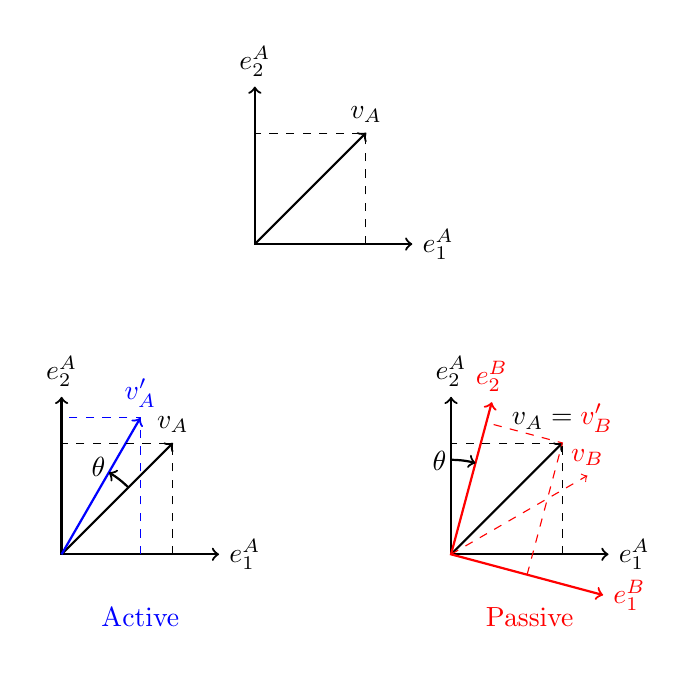
\begin{tikzpicture}[scale=2]
  % Draw axes
  \matrix[column sep=-5mm, row sep=10mm] {
    &
    {
            \draw [<->,thick] (0,2) node (yaxis) [above] {$e_{2}^{A}$}
      |- (2,0) node (xaxis) [right] {$e_{1}^{A}$};
      \draw [rotate=45,->,thick] (0,0)--(2,0) node [above] {$v_{A}$};
      \draw [dashed] (1.41,0) |- (0,1.41);
    }
&
\\
    {
      \draw [<->,thick] (0,2) node (yaxis) [above] {$e_{2}^{A}$}
      |- (2,0) node (xaxis) [right] {$e_{1}^{A}$};
      \draw [rotate=45,->,thick] (0,0)--(2,0) node [above] {$v_{A}$};
      \draw [rotate=60,->,thick,blue] (0,0)--(2,0) node [above] {$v'_{A}$};
      \draw [dashed] (1.41,0) |- (0,1.41);
      \draw [dashed,blue] (1,0) |- (0,1.732);
      \draw [rotate=-30,<-,thick] (0,1.2) arc (90:75:1.2cm) node at (97:1.2) {$\theta$};
      \node [blue] at (1,-0.8) {Active};
    }
&
&
    % Draw axes
    {
      \draw [<->,thick] (0,2) node (yaxis) [above] {$e_{2}^{A}$}%
      |- (2,0) node (xaxis) [right] {$e_{1}^{A}$};
      \draw [rotate=45,->,thick] (0,0)--(2,0) node [above]%
            {$v_{A} \color{black}= \color{red}v'_{B}$};
      \draw [rotate=30,->,dashed,red]  (0,0)--(2,0) node [above] {$v_{B}$};
      \draw [rotate=-15,<->,thick,red] (0,2) node (yaxis) [above] {$e_{2}^{B}$}%
      |- (2,0) node (xaxis) [right] {$e_{1}^{B}$};
      \draw [dashed] (1.41,0) |- (0,1.41);
      %\draw [rotate=-15,dashed,red] (1.41,0) |- (0,1.41);
      \draw [rotate=-15,dashed,red] (1,0) |- (0,1.732);
      \draw [->,thick] (0,1.2) arc (90:75:1.2cm) node at (97:1.2) {$\theta$};
      \node [red] at (1,-0.8) {Passive};
    }
\\
  };
\end{tikzpicture}

\end{document}
